\documentclass[12pt,a4paper]{article}
\usepackage[utf8]{inputenc}
\usepackage{amsmath}
\usepackage{amsfonts}
\usepackage{amssymb}
\usepackage{graphicx}
\usepackage{array}
\usepackage{listings}
\begin{document}
\lstset{language=Java}
\section{Suche}\label{search}
Baguette verwendet eine sequentielle, rekursive Suche auf Grundlage von Min/Max Algorithmus und Alpha/Beta Pruning, um beste Züge aus dem parallel generierten Suchbaum zu finden.
Die Suche wird wiederholt, bei erreichen neuer tiefen im Suchbaum gestartet, es handelt sich dabei also um eine iterative suche.

\subsection{Min/Max Algorithmus}
Der Minimax-Algorithmus ist ein grundlegendes verfahren um einen besten Zug aus dem Suchbaum zu finden. Der minimierende Spieler ist dazu bestrebt den Zug mit niedrigstem Wert zu wählen. Der maximierende Spieler ist bestrebt den Zug mit dem höchsten Wert zu wählen.
Diese Werte werden dabei bis zur Wurzel getragen, bei welcher dann entsprechend der beste Zug für den jeweils am Zug befindlichen Spieler gewählt wird. Durch dieses Prinzip wählt der am Zug befindliche Spieler also immer den Zug mit dem geringsten Schaden bzw den Zug mit dem größten Vorteil. Eine Vorbedingung für ein sinnvolles Ergebnis des Minimax-Algorithmus ist, dass alle Blattknoten im Suchbaum auf der selben Tiefe liegen, da höher liegende Knoten sonst tiefer liegende Knoten verdecken würden.  
\\\\
Beispiel:\\Jeder Knoten stellt einen möglichen Zug dar.
\begin{figure}[h]
\begin{center}
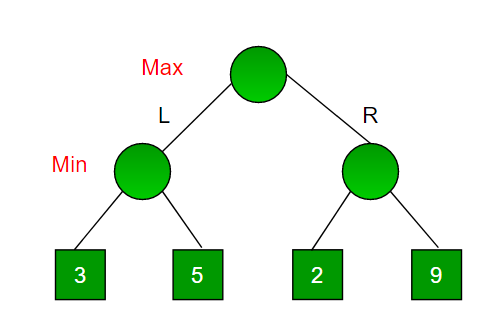
\includegraphics[scale=0.5]{minmax.png}
\caption{source: www.geeksforgeeks.org/minimax-algorithm-in-game-theory-set-1-introduction}
\end{center}
\end{figure}

Wir beginnen bei dem minimierenden Knoten links.
Dieser wählt das Minimum zwischen 3 und 5, also 3.
Dieser Knoten hat also nun den Wert 3.\\
Gehen wir nun zum minimierenden Knoten Rechts über.
Dieser wählt das Minimum zwischen 2 und 9, also 2.
Dieser Knoten hat also nun den Wert 2.
Als letztes betrachten wir den maximierenden Knoten und somit gleichzeitig die Wurzel.
Dieser wählt das Maximum zwischen 3 und 2, also 3.
Der beste Zug der an der Wurzel gewählt werden kann ist also der rechte.

\section{Alpha/Beta Pruning}
Alpha/Beta Pruning ist eine Erweiterung des Minimax-Algorithmus, durch die nicht alle Knoten im Suchbaum betrachtet werden müssen. Dadurch kann, bei gleich bleibendem Ergebnis, Zeit eingespart werden und somit tiefere Ebenen im Suchbaum erreicht werden.
\\\\
Prinzip anhand eines Beispiels.
Die Berechnung des besten Wertes für folgenden Suchbaum sieht wie folgt aus:
\begin{flushleft}
max\{ min\{3,5,10\}, min\{2,a,b\}, min\{2,7,3\}\}\\ = max\{3,c,2\}\\ = 3      $$a,b,c \in \mathbb{N}$$
\end{flushleft}
3 ist dabei das richtige Ergebnis, da unabhängig von a und b, $c<=2$ sein muss. In Worten bedeutet das, dass der Zug mit den Unbekannten nicht weiter durchsucht werden muss, da er durch den wert 2 bereits schlechter werden kann als der linke Zug mit wert 3. 

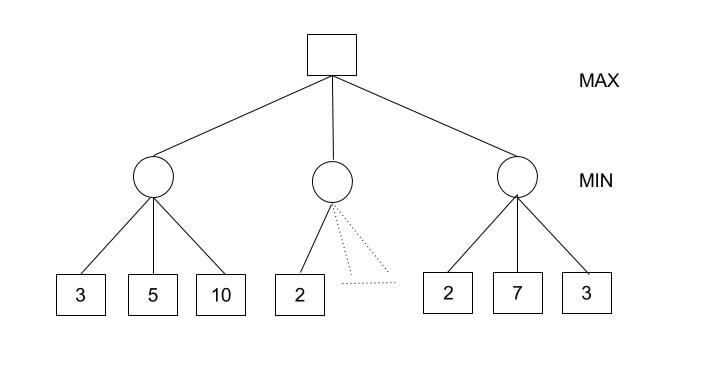
\includegraphics[scale=0.5]{alpha-beta-pruning.jpg}\\
\begin{tiny}
Beispiel und Bild entnommen von: hackerearth.com/blog/developers/minimax-algorithm-alpha-beta-pruning
\end{tiny}\\
Alpha und Beta sind die Namen der variablen , die verwendet werden um zu überprüfen ob der Wert eines Knotens bereits schlechter ist als der eines vorher besuchten Knotens. Alpha wird nur vom maximierenden Spieler verändert und Beta nur vom minimierenden Spieler.
Wenn Alpha größer als Beta ist kann die suche auf dem aktuellen Knoten abgebrochen werden.
\\\\
Hierzu vereinfachter code der Alpha/Beta Funktion wie sie in Baguette verwendet wird. Da die Funktion selbst nur eine Wert zurück gibt, wird in der letzten if Bedingung zusätzlich die globale BestMove Variable mit dem gefundenen besten Zug gesetzt, wenn der aktuell untersuchte Knoten die Wurzel des Suchbaum ist.
\begin{lstlisting}[frame=single]
int alphaBetaSearch(parent, maxDepth, alpha, beta) {
        bestValue = parent.blacksTurn() ?
                MAX_VALUE : MIN_VALUE;

        if (parent.getDepth() == maxDepth) {
            return parent.getValue();
        } else {
            for (int i = 0; i < children.length; i++) {
                curValue = alphaBetaSearch
                (children[i], maxDepth, alpha, beta);

                if (parent.blacksTurn()) {
                    if (curValue < bestValue) {
                        bestValue = curValue;
                        beta = curValue;
                        bestMove = children[i];
                    }
                } else {
                    if (curValue > bestValue) {
                        bestValue = curValue;
                        alpha = curValue;
                        bestMove = children[i];
                    }
                }
                if (beta <= alpha) {
                    break;
                }
            }
            if (parent == ROOT) {
                setBestMove(bestMove);
            }
         return bestValue;
\end{lstlisting}

\end{document}